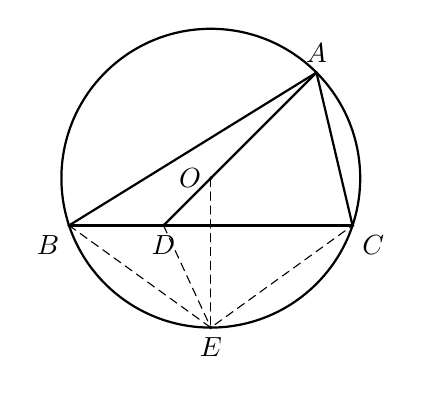
\begin{tikzpicture}[line cap=round,line join=round,scale=0.6]
\pgfmathsetmacro{\sfive}{sqrt(5)}
\pgfmathsetmacro{\R}{sqrt(10)}

\coordinate (B) at (-3,0);
\coordinate (C) at (3,0);
\coordinate (D) at (-1,0);
\coordinate (O) at (0,1);                 % 让 O 在 AD 上（按构造选取）
\coordinate (A) at (\sfive,{1+\sfive});   % 同时保证 A,B,C 共圆（圆心 O，半径 sqrt(10)）
\coordinate (E) at (0,{1-\R});            % 圆的最低点（示意）

\draw[thick] (O) circle (\R);

\draw[thick] (B)--(C);
\draw[thick] (A)--(B);
\draw[thick] (A)--(C);
\draw[thick] (A)--(D);

\draw[densely dashed] (B)--(E)--(C);
\draw[densely dashed] (D)--(E);
\draw[densely dashed] (O)--(E);

\fill (A) circle (1.1pt);
\fill (B) circle (1.1pt);
\fill (C) circle (1.1pt);
\fill (D) circle (1.1pt);
\fill (E) circle (1.1pt);
\fill (O) circle (1.1pt);

\node[above] at (A) {$A$};
\node[below left] at (B) {$B$};
\node[below right] at (C) {$C$};
\node[below] at (D) {$D$};
\node[below] at (E) {$E$};
\node[left] at (O) {$O$};
\end{tikzpicture}